\subsection{Design Principles} \label{sec:design-principles}

OlaVM's vision is to build a high-performance, programmable and decentralized Ethernet scaling solution that can help the Ethereum ecosystem to
host more businesses and applications in the future. See \figref{fig:olavm-vision}.
\begin{itemize}
    \item As Layer2, it needs to achieve high performance while taking into account the core features of programmability, composability and
          decentralization, so that existing and future Ethereum applications can be directly deployed on OlaVM;
    \item Higher throughput and lower cost are the demands of these applications
\end{itemize}
You can read \href{https://vitalik.ca/general/2022/09/17/layer_3.html}{Vitalik: What kind of layer 3s make sense?} and
\href{https://medium.com/starkware/fractal-scaling-from-l2-to-l3-7fe238ecfb4f}{Starkware: Fractal Scaling: From L2 to L3} for more discussion
on Layer2, Layer3 features and scenarios.

\begin{figure}[!ht]
    \centering
    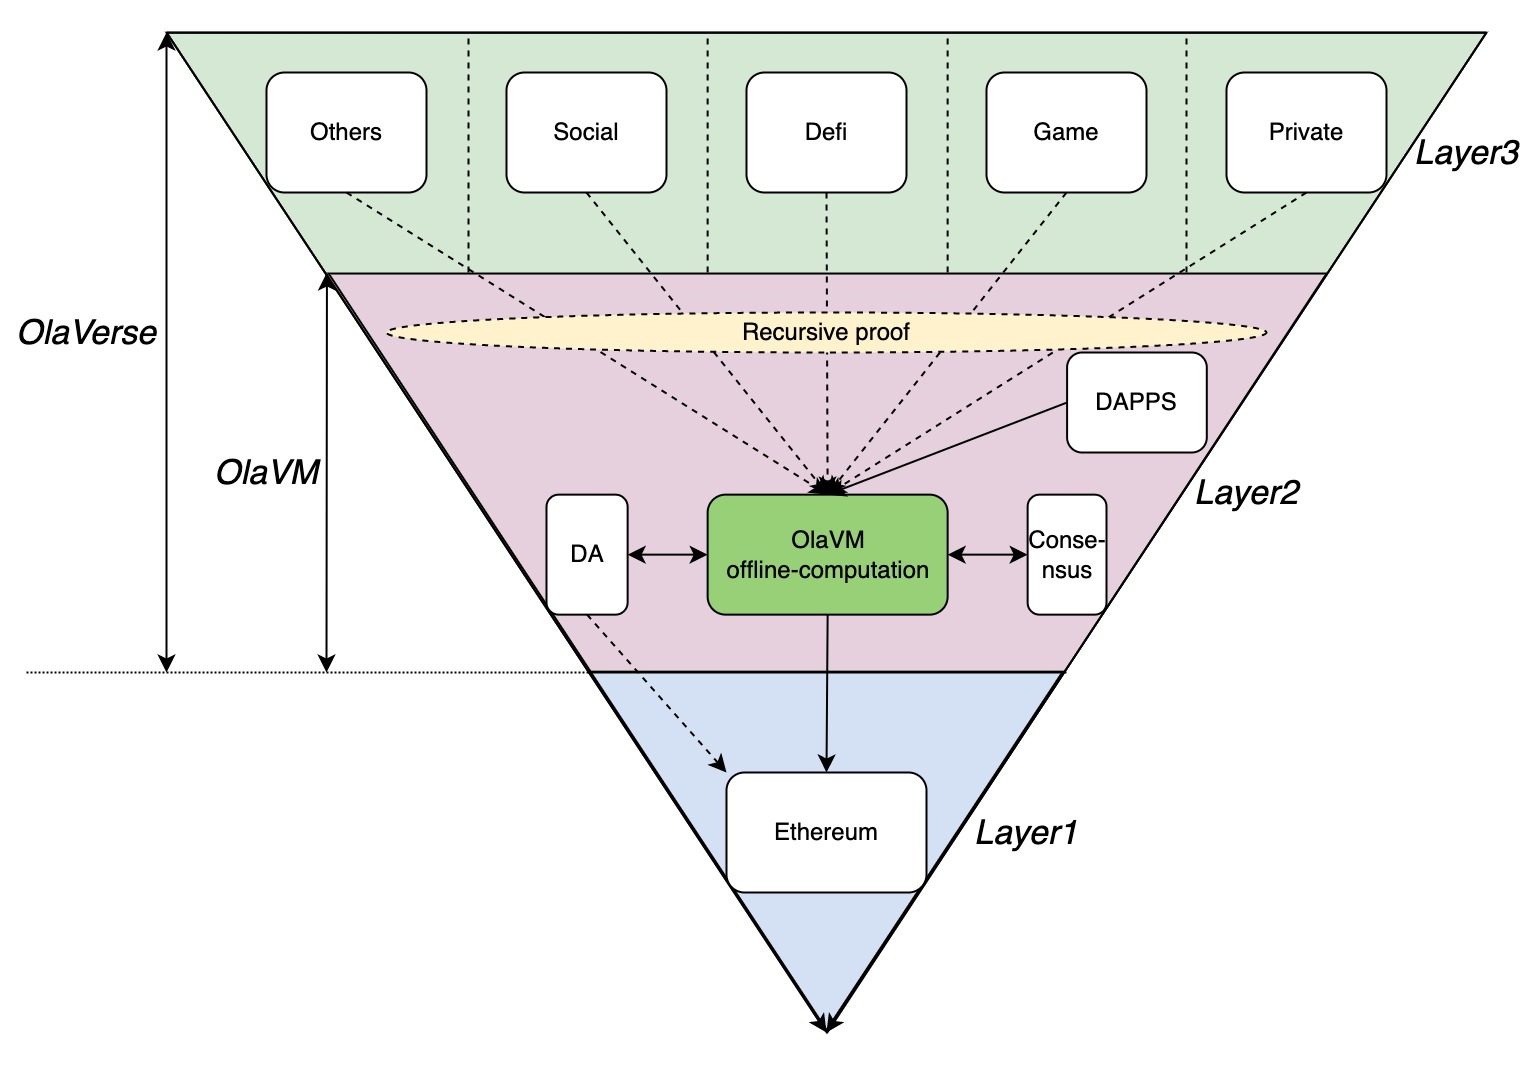
\includegraphics[width=0.8\textwidth]{vm/olavm-vision.jpeg}
    \caption{OlaVM's vision}
    \label{fig:olavm-vision}
\end{figure}

\subsubsection{Design of Instruction Set} \label{sec:design-instruction-set}

OlaVM uses the Reduced Instruction Set Computer (RISC) architecture, one of its main features is a small instruction set, as opposed to the Complex Instruction Set Computer (CISC) architecture.
The difference between the two can be found in \href{https://cs.stanford.edu/people/eroberts/courses/soco/projects/risc/risccisc/}{RISC vs. CISC}.

\emph{1. A reduced instruction set reduces the number of constraint polynomials}

In ZKVM, there is a very critical constraint, the CSTC (CPU State Transition Constraint); it is mainly used to constrain the validity
of VM state changes before and after the execution of an instruction.

\begin{figure}[!ht]
    \centering
    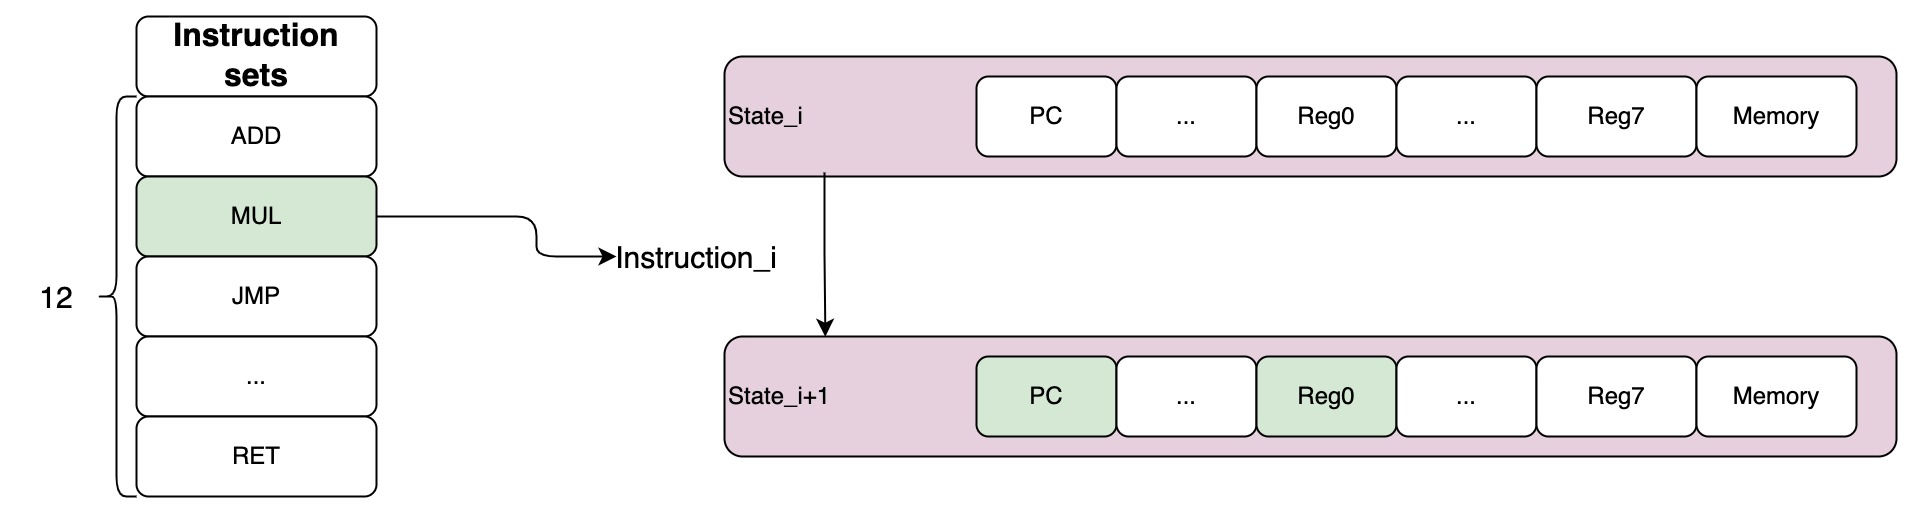
\includegraphics[width=0.7\textwidth]{vm/olavm-instruction-state.jpeg}
    \caption{Instruction-induced cpu state transition}
    \label{fig:instruction-cpu-state-transition}
\end{figure}

As shown in \figref{fig:instruction-cpu-state-transition}, there are many registers in the VM. When VM executes an instruction, it will
cause the state of some registers to change, so to ensure the correctness of VM execution, we need to constrain:
\begin{itemize}
    \item The change of register state involved in the execution of the instruction is valid;
    \item The status of registers not involved in the instruction execution remains unchanged.
\end{itemize}

Let's look at a simple example to explain the constraints on register state changes:
\begin{table}[!ht]
    \centering
    \begin{tabular}{|c|c|c|c|c|c|c|c|}
        \hline
        \rowcolor{gray} clk & pc    & instruction        & \dots & reg0  & reg1  & reg2  & \dots \\
        \hline
        \dots               & \dots & \dots              & \dots & \dots & \dots & \dots & \dots \\
        \hline
        78                  & 8     & ADD reg0 reg0 reg1 & \dots & 1     & 2     & 0     & \dots \\
        \hline
        79                  & 9     & MOV reg2 3         & \dots & 3     & 0     & 0     & \dots \\
        \hline
        80                  & 11    & JMP 2              & \dots & 3     & 0     & 3     & \dots \\
        \hline
        81                  & 2     & \dots              & ...   & 3     & 0     & 3     & \dots \\
        \hline
    \end{tabular}
    \caption{Example of cpu state transitions}
    \label{table:example-cpu-state-transitions}
\end{table}

\tabref{table:example-cpu-state-transitions} briefly presents the changes of some registers after the VM executes three
instructions; taking the PC register as an example, the logic of the updates of the three instructions are:
\begin{itemize}
    \item ADD: $\mathrm{pc}_{i+1} = \mathrm{pc}_i + 1$
    \item MOV: $\mathrm{pc}_{i+1} = \mathrm{pc}_i + 2$
    \item JMP: $\mathrm{pc}_{i+1} = 2$
\end{itemize}

From the point of view of constraints, we do not know which instruction the VM is going to execute each time, so we have to
design a constraint that can handle all instructions, which we call (CSTC) CPU State Transition Constraint.For the simple
example above, we can design the update logic of the PC as follows:
\[ \mathrm{pc}_{i+1} = \mathrm{sel\_jmp}_i \cdot \mathrm{imm\_value} + (1 - \mathrm{sel\_jmp}) \cdot (\mathrm{pc}_i + 1 + \mathrm{op1\_imm}) \]

We write all state transitions of the cpu in this constrained form.The addition of each instruction adds new selectors resulting
in increased constraint complexity, so we limit the size of instructions to 19 (including builtins).

Of course, even though we have a reduced instruction set architecture, we still need to maintain the Turing-complete feature so that
we can still compute everything based on these simple instruction sets.So that based on these simple instruction sets, we can still
compute everything that can be computed. Based on these instructions, combined with the prophet mechanism in Section \ref{sec:design-prophet}, we build a Turing-complete
language, Ola-lang, that supports loops and recursive operations.

\emph{2. Most of the operations will use a small part of the instruction set}

Under the CISC architecture, a large instruction set is defined. However, in reality, each instruction is used differently and for most
of the computations, only a small part of the instruction set may be used.From the constraint point of view, this is a big waste because
the constraint logic of all instructions needs to be included in the constraint system (CSTC), and the worst case would be that each instruction
would correspond to a constraint factor, thus making the whole constraint scale complex, including the number of polynomials and the order of
the constraints.

\begin{figure}[!ht]
    \centering
    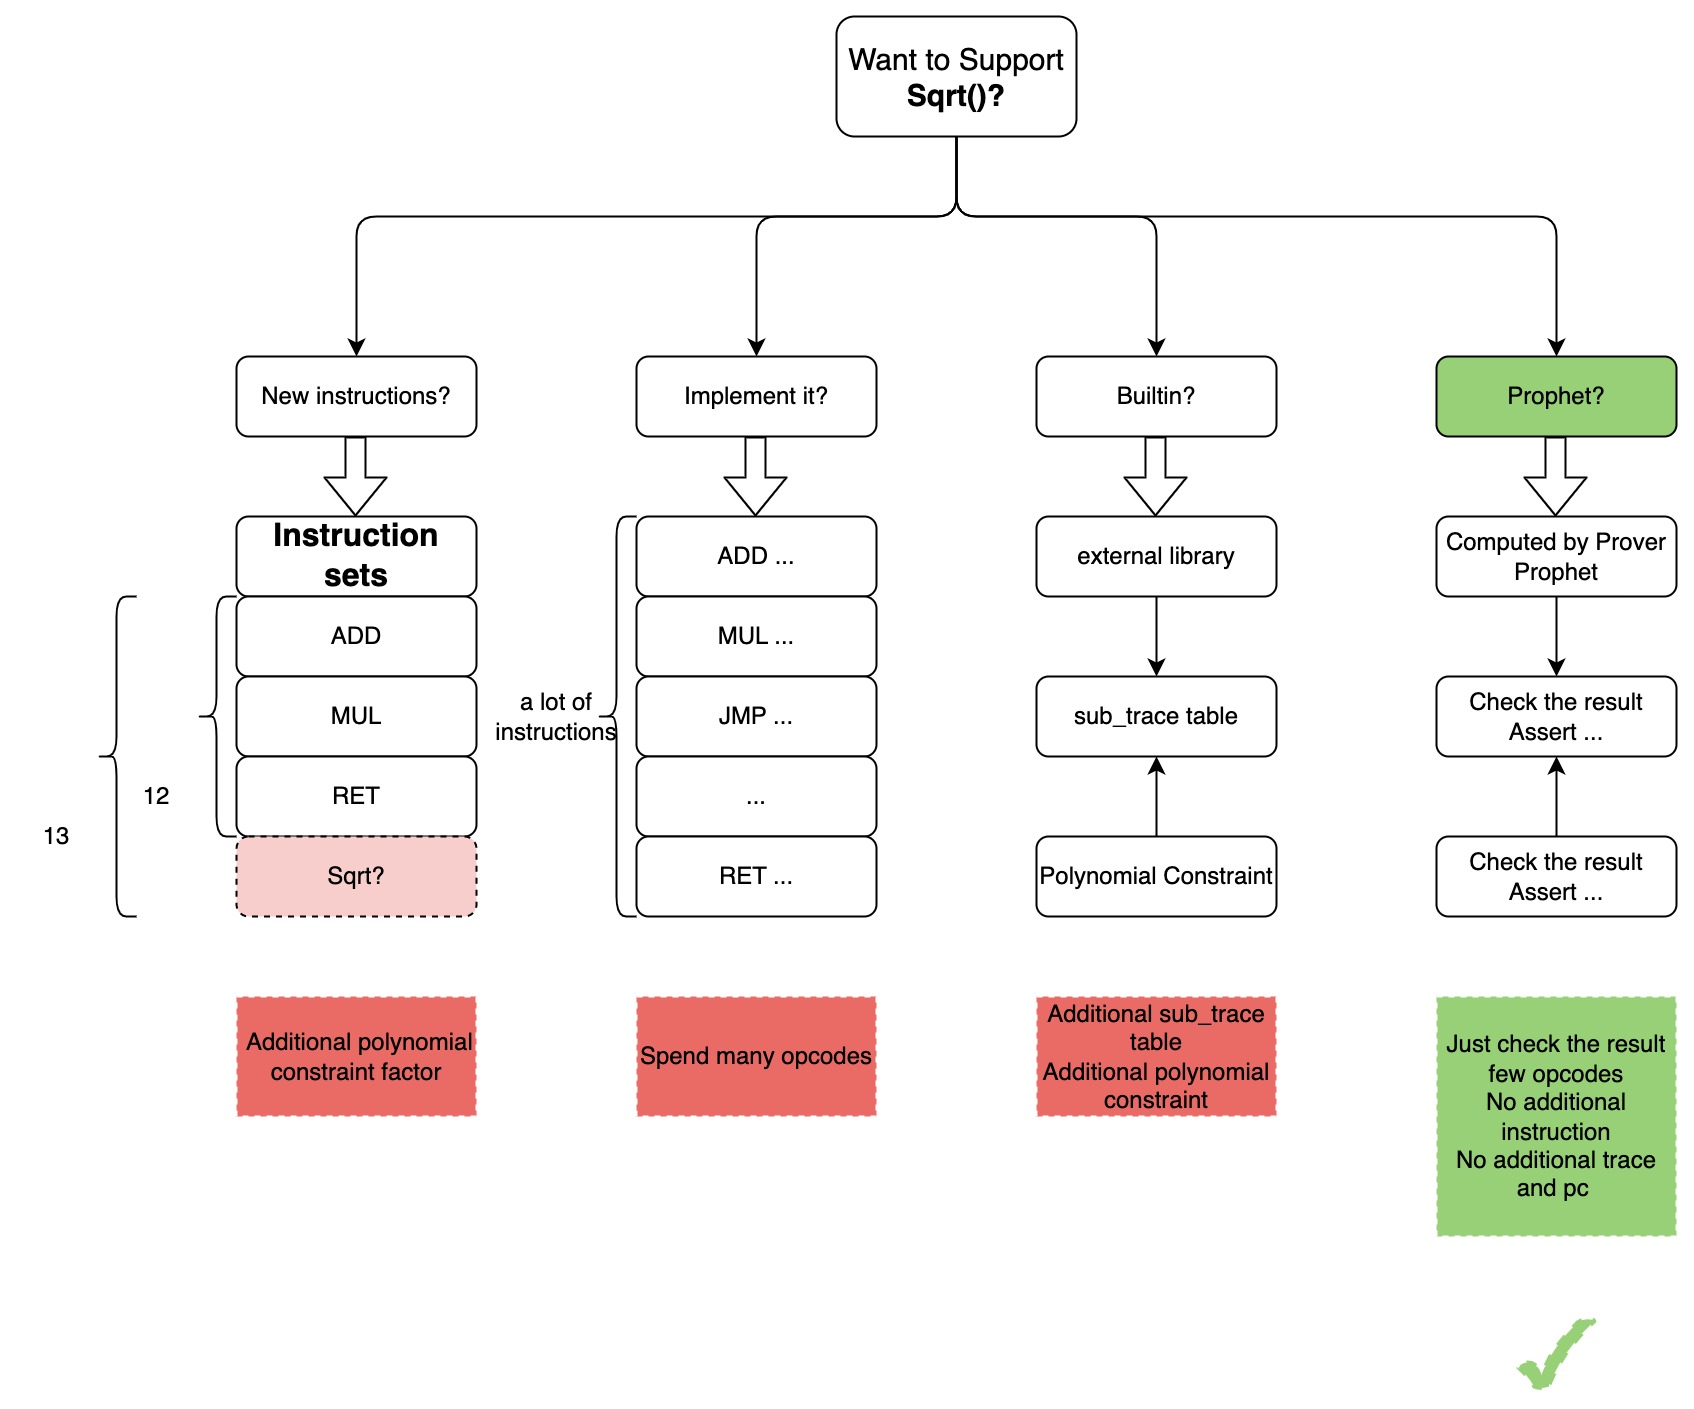
\includegraphics[width=0.6\textwidth]{vm/design-support-zk-unfriendly.jpeg}
    \caption{The best way to support ZK-Unfriendly computation}
    \label{fig:desgin-support-zk-unfriendly}
\end{figure}

For some calculations, in many cases, we prefer to use the existing instruction set rather than introduce a new instruction; 
although this will make the program bigger (more opcodes), some redundant data will be added during the verification itself to
facilitate doing the FFT; but if it is a complex computation that requires a particularly large number of instructions to implement, we still
have ways to solve it, such as introducing Builtins and Prophet, whose principles we will focus on in later chapters, where you just need to
know that they can help drastically reduce the consumption of instructions to implement these complex computations, as shown in \figref{fig:desgin-support-zk-unfriendly}.

\subsubsection{Design of Registers} \label{sec:design-registers}

As mentioned in chapter \ref*{sec:design-instruction-set}, in ZKVM, we not only have to constrain the state of the registers associated with
the instruction to be updated correctly, but we also have to constrain the state of the registers not involved in the current
instruction to remain unchanged.Even though register-based VMs have certain advantages, from the verification point of view,
it is not better to have a larger number of registers;there is a trade-off to be considered:

\begin{itemize}
    \item How many registers will be sufficient for most of the calculations?
    \item For some calculations, is the increased number of memory accesses acceptable when there are not enough registers?
\end{itemize}

If the number of registers is small enough and at the same time the memory accesses introduced do not yet need to be constrained,
this would be the ideal case from the point of view of verification efficiency, as in the design of the Cairo VM, where there are
no general-purpose registers and all operands of the instruction originate from memory;at the same time, to avoid consistency checks
on memory, the write-once model is used, since memory cannot be rewritten at the execution level, so checks are not needed.

However, the downside of introducing the write-once model is that DSLs are not friendly to Dapps developers, and the limitations of
the memory model make it necessary for developers to pay special attention to the way memory is used when developing Dapps with DSLs
(the traditional memory model is the read-write model).

\begin{figure}[!ht]
    \centering
    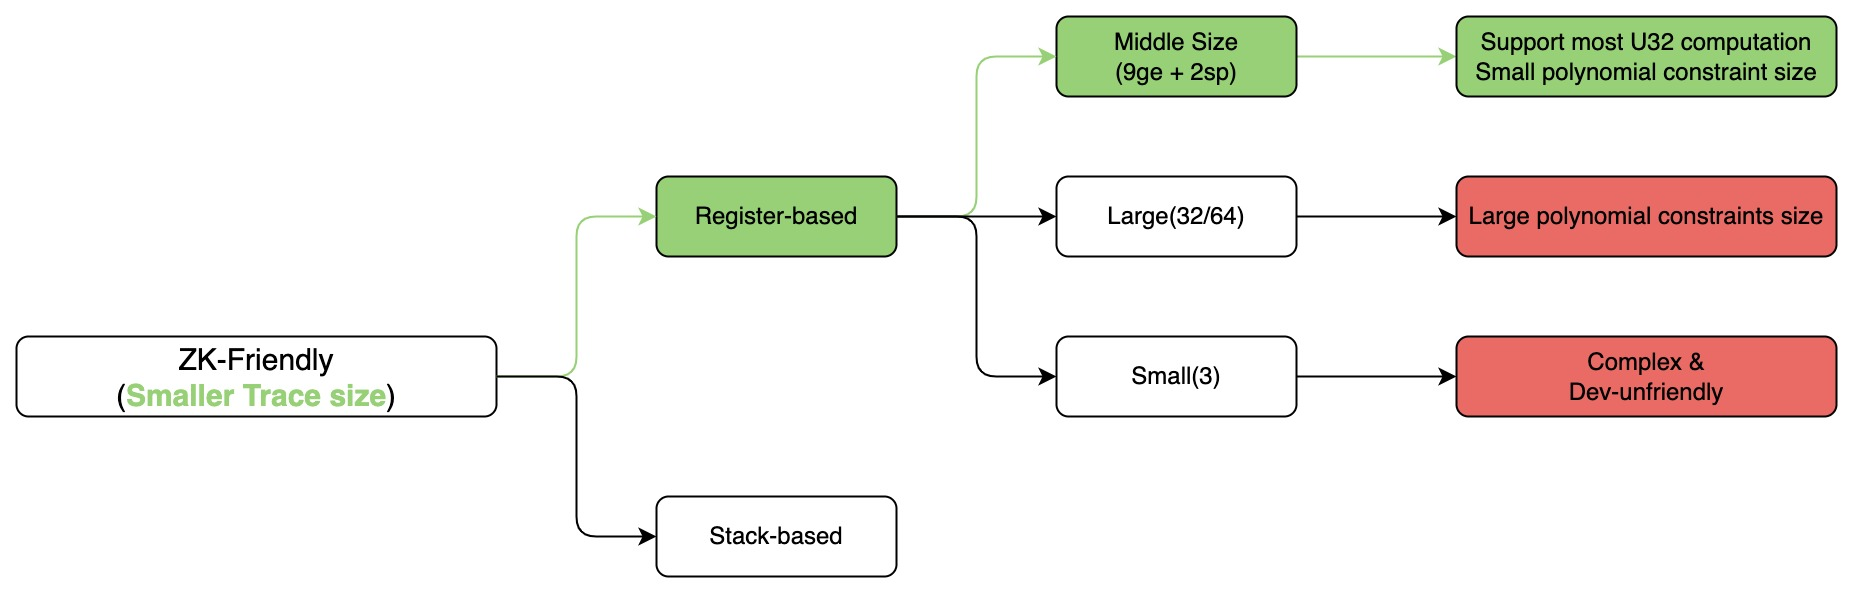
\includegraphics[width=0.8\textwidth]{vm/design-zk-friendly-register.jpeg}
    \caption{How to get ZK-Friendly(Smaller Trace) from register}
    \label{fig:design-zk-friendly-register}
\end{figure}

As shown in \figref{fig:design-zk-friendly-register}, we choose an optimal solution from both ZK-Friendly and Dev-Friendly perspectives.In terms of the number of
registers, considering that the minimum type of computation supported on OlaVM is U32 integer computation, plus some boundary conditions,
such as the number of loops, loop termination conditions, etc, nine general-purpose registers can support most of the U32 computation
(both U64 and U256 integer computation can be implemented through the U32 library), and 2 system registers(PC, PSP) is used in OlaVM, reference: \ref{subsubsec: zkvm-executor-register}. 
When the number of registers is not enough, memory is needed for caching, so memory access-related instructions
(MLOAD, MSTORE) will be added, but it is worth noting that in order to facilitate the FFT, Prover often adds redundant data in Trace to meet
the size of Trace to the power of 2.be replaced with valid data, as shown in \figref{fig:design-better-trace-layout}

\begin{figure}[!ht]
    \centering
    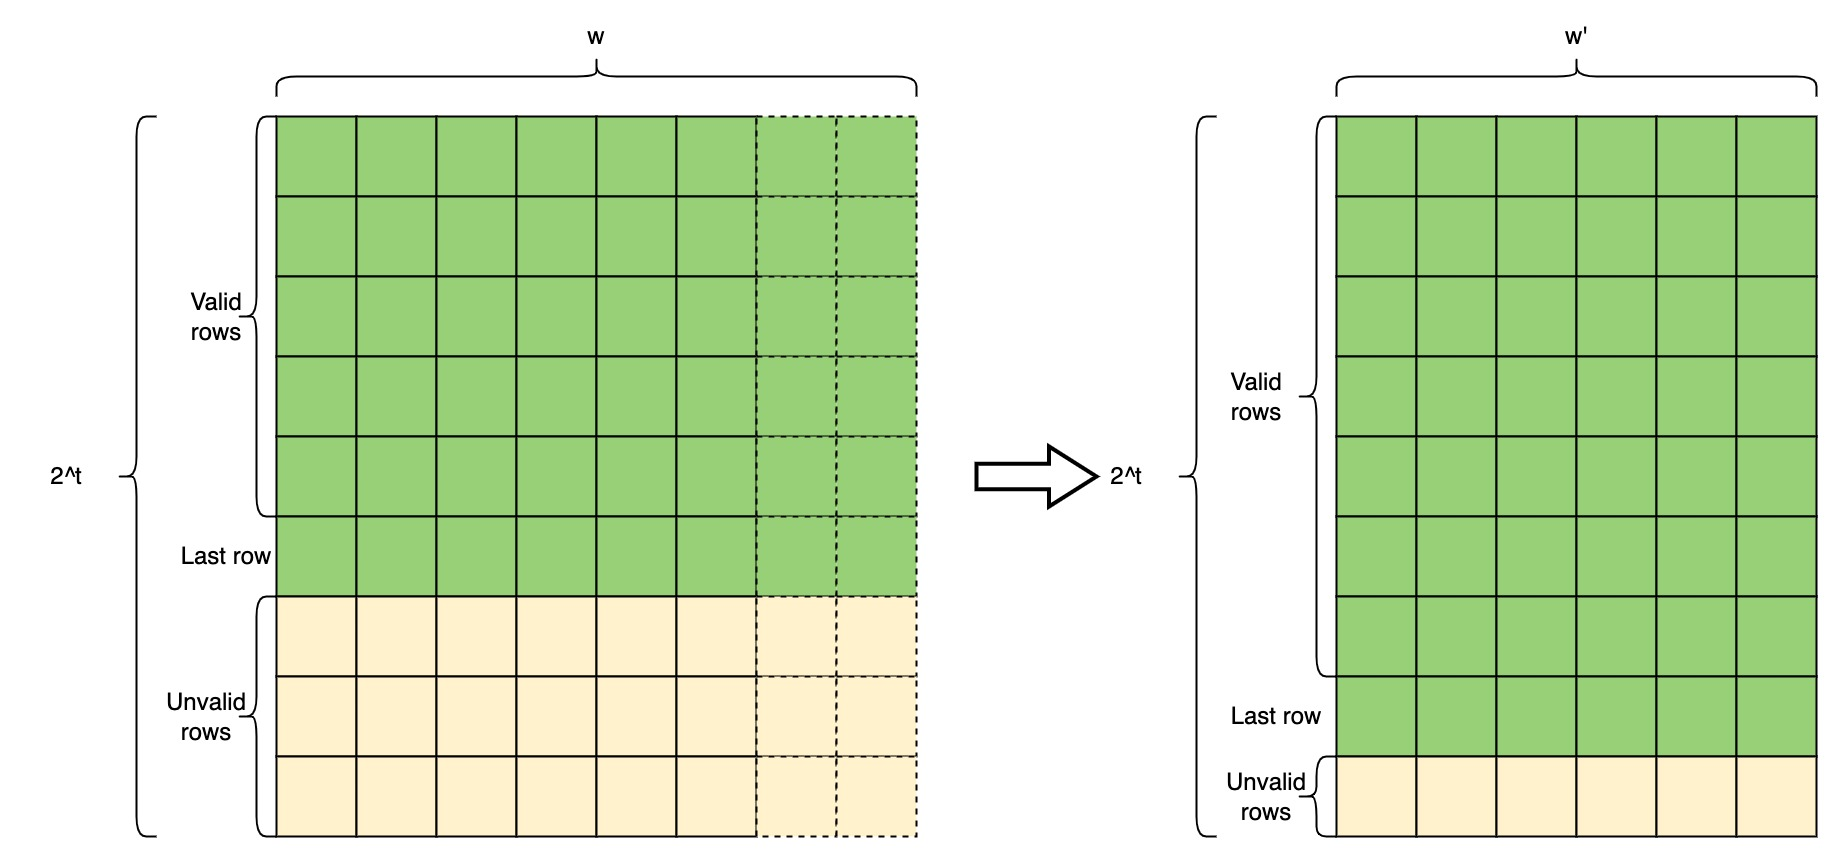
\includegraphics[width=0.8\textwidth]{vm/design-better-trace-layout.jpeg}
    \caption{Better layout of Trace}
    \label{fig:design-better-trace-layout}
\end{figure}